\documentclass[review]{./elsarticle}

\usepackage{lineno,hyperref}
\modulolinenumbers[5]

\journal{Journal of \LaTeX\ Templates}

%%%%%%%%%%%%%%%%%%%%%%%
%% Elsevier bibliography styles
%%%%%%%%%%%%%%%%%%%%%%%
%% To change the style, put a % in front of the second line of the current style and
%% remove the % from the second line of the style you would like to use.
%%%%%%%%%%%%%%%%%%%%%%%

%% Numbered
%\bibliographystyle{model1-num-names}

%% Numbered without titles
%\bibliographystyle{model1a-num-names}

%% Harvard
%\bibliographystyle{model2-names.bst}\biboptions{authoryear}

%% Vancouver numbered
%\usepackage{numcompress}\bibliographystyle{model3-num-names}

%% Vancouver name/year
%\usepackage{numcompress}\bibliographystyle{model4-names}\biboptions{authoryear}

%% APA style
%\bibliographystyle{model5-names}\biboptions{authoryear}

%% AMA style
%\usepackage{numcompress}\bibliographystyle{model6-num-names}

%% `Elsevier LaTeX' style
\bibliographystyle{elsarticle-num}

\usepackage{color}
\usepackage{subcaption}
\usepackage{graphicx}
\usepackage{booktabs} % nice rules for tables
\usepackage{microtype} % if using PDF
\usepackage{xspace}
\usepackage{listings}
\usepackage{textcomp}
\usepackage{multicol,tabularx,capt-of}
\usepackage{multirow}
\usepackage{pdflscape}

\newcommand{\code}[1]{\lstinline[basicstyle=\ttfamily\color{green!40!black}]|#1|}
\newcommand{\units}[1] {\:\text{#1}}%
\newcommand{\SN}{S$_N$}
\newcommand{\cyclus}{\textsc{Cyclus}\xspace}
\newcommand{\Cyclus}{\cyclus}
\newcommand{\citeme}{\textcolor{red}{CITE}\xspace}
\newcommand{\TODO}[1] {{\color{red}\textbf{TODO: #1}}}%

\newcommand{\comment}[1]{{\color{green}\textbf{#1}}}

\usepackage[acronym]{glossaries}
%\makeglossaries
%%%%%%%%%%%%%%%%%%%%%%%%%%%%%%%%%%%


\newacronym{FBR}{FBR}{fast breeder reactor}
\newacronym{HEU}{HEU}{Highly Enriched Uranium}
\newacronym{IAEA}{IAEA}{International Atomic Energy Agency}
\newacronym{LEU}{LEU}{Low Enriched Uranium}
\newacronym{LWR}{LWR}{light water reactor}
\newacronym{MOX}{MOX}{mixed oxide fuel}
\newacronym{SQ}{SQ}{significant quantity}
\newacronym{UOX}{UOX}{uranium oxide fuel}
%%%%%%%%%%%%%%%%%%%%%%%%%%%%%%%%%%%
%%%%%%%%%%%%%%%%%%%%%%%

\begin{document}

\begin{frontmatter}

    
%% Group authors per affiliation:
\author{Baptiste Mouginot\corref{mycorrespondingauthor}}
\ead{mouginot@wisc.edu}

\author{Kathryn Mummah}
\ead{mummah@wisc.edu}

\author{Jordan Stomps}
\ead{stomps@wisc.edu}

\author{Paul P.H. Wilson}
\ead{paul.wilson@wisc.edu}

\address{Department of Engineering Physics, University of Wisconsin-Madison}

\cortext[mycorrespondingauthor]{Corresponding author}
%% or include affiliations in footnotes:
%\author[mymainaddress,mysecondaryaddress]{Elsevier Inc}
%\ead[url]{www.elsevier.com}

%\author[mysecondaryaddress]{Global Customer Service\corref{mycorrespondingauthor}}
%\ead{support@elsevier.com}




\date{\today}

\title{Evaluating computational methods for modeling off-normal operation of gas centrifuge cascades}
%tnotetext[mytitlenote]{Fully documented templates are available in the elsarticle package on \href{http://www.ctan.org/tex-archive/macros/latex/contrib/elsarticle}{CTAN}.}


% 0.Abstract

\begin{abstract}
\begin{itshape}
This work compares and evaluates different computational approaches for modeling
off-normal operation of a gas centrifuge enrichment cascade.

The goal of this work focuses on developing the necessary understanding of
potential misuse of enrichment cascades, contributing to more effective
international safeguards designs and approaches.  While it is straightforward to
design a symmetric enrichment cascade under ideal conditions as a function of the
theoretical feed, product, and tails assays, it is very difficult to find
reliable information about the behavior of a given cascade when the feed assay
does not match the design value. Several methods have been developed to assess
the behavior of an enrichment cascade in such circumstances. In addition to the
cut, ($\theta$) these methods evaluate the feed-to-product, feed-to-tails, and the
product-to-tails enrichment ratio, $\alpha$, $\beta$ and $\gamma$, respectively,
as a function of the cascade feed assay. As those four parameters depend on each
other, determining two of them fully defines the other.  The first approach
consists of fixing $\theta$ and $\alpha$, recomputing the corresponding assays at
each stages of the cascade. The second one maintains the ideal condition of the
cascade ($\alpha$ and $\beta$ fixed across the whole cascade), modifying
$\theta$ values at each stage accordingly. Both approaches have been implemented
into the \Cyclus fuel cycle simulator\cite{cyclus, mbmore.2018}. The third fixes
$\theta$ and $\gamma$, using both $\alpha$ and $\beta$ at each stage as free
parameters. The third method has been investigated in \cite{walker.2017}.

Following a description of each method and an evaluation of differences between
each approach, this work compares the results produced by these methods within
scenarios involving misuse of symmetric enrichment cascades simulated using the dynamic
nuclear fuel cycle simulator, \Cyclus.
\end{itshape}

\end{abstract}


%\begin{keyword}
%\texttt{elsarticle.cls}\sep \LaTeX\sep Elsevier \sep template
%\MSC[2010] 00-01\sep  99-00
%\end{keyword}

\end{frontmatter}

\linenumbers

\maketitle


% I.   Motivation
\section{Motivation}

Gas centrifuge cascades are usually designed to operate in an ideal manner, with
no losses in separative work. To achieve such ideal configuration, the cascade
is designed to be fed with a specific feed assay and produce the target
enrichment while rejecting tails at a fixed assay.

With the current international tensions regarding enrichment capabilities, this
work aims to measure the effectiveness of a symmetric enrichment cascade when
used outside of its designed scope and to quantify the attractiveness %Katie: I would be VERY VERY careful using the word attractiveness.
of such ways
to build up a \gls{SQ} of \gls{HEU}, defined by the \gls{IAEA} as \(25 \ kilograms\)\cite{noauthor_iaea_2001}.

The present work investigates the performance of an enrichment cycle when chaining
gas centrifuge enrichment cascades tuned for \gls{LEU} production from natural uranium to instead produce \gls{HEU}. Literature on the subject is limited due to its
internationally and politically sensitive nature. Three behavior models have been
implemented and used to evaluate the response of an enrichment cascade when fed
with different assays than originally designed. This work also takes advantage
of the \Cyclus \cite{cyclus} fuel cycle simulator's capabilities to evaluate the
assay values at equilibrium.


% II.  Theory
%   a. cascade design
%   b. misuse model
%       i.   case A
%       ii.  case B
%       iii. case C
\section{Theory}

In the following section, equations and algorithms used to model the behavior of
a symmetric ideal gas centrifuge cascade from individual centrifuge properties
are described. Details will also be provided to model centrifuge behavior
when fed with a different feed enrichment than designed.

\subsection{Centrifuge properties}

\subsubsection{Separative power}

\paragraph{R\"aetz equation}

As described by Glaser in \cite{glaser.2008}, the separative power of a single centrifuge can be express as an analytical solution \cite{raetz.phd} of the
differential equation for the gas centrifuge:

\begin{eqnarray}
    \label{eq:raetz}
    \delta U(L,F,\theta,Z_{p}) &= &\frac{1}{2}
            F\theta(1 - \theta)
            \left(\frac{\Delta M}{2 RT}v_{a}^{2}\right)^{2}
            \left(\frac{r_{2}}{a}\right)^{4}
            \left[1 - \left(\frac{r_{1}}{r_{2}}\right)^{2}\right]^{2}
            \label{eq_raetz}\\
        &&
            \left[
                \left(\frac{1+L/F}{\theta}\right)
                (1- exp[ - A_{P}(L,F,\theta)Z_{p}])  \nonumber  \right. \\
        &&~~ + \left.\left(\frac{L/F}{1 - \theta}\right)
                (1 - exp[ -A_{W}(L,F,\theta)(Z - Z_{p}])\right]^{2}, \nonumber
                \\
    \textrm{with~ ~ ~ ~ ~}
        A_{P} &= &\frac{2\pi D\rho }{ ln(r_{2}/r_{1}) }
                 \frac{ 1 }{ F }
                 \frac{ 1-\theta }{(1+L/F)(1-\theta+L/F) }\\
        A_{W} &= &\frac{2\pi D\rho }{ ln(r_{2}/r_{1}) }
                 \frac{ 1 }{ F }
                 \frac{ 1-\theta }{ (L/F)(1-\theta+L/F) }
\end{eqnarray}

In this equation, the parameters of average gas temperature, $T$, peripheral speed,
$v_a$, height, $h$, diameter, $d$, pressure ratio, $x$, feed flow rate, $F$,
counter-current flow ratio, $L/F$, are intrinsic to the centrifuge design.
To match the cascade design describe in \cite{glaser.2008} and \cite{walker.2017},
P1-type centrifuge properties have been chosen (Table \ref{tab:centrifuges}).

\begin{table}[htb]
    \centering
    \caption{Summary of the centrifuge parameters.}
    \begin{tabular}{ccccccc}
        \toprule
        $T$[K] & $v$[m/s] & $h$[m] & $d$[m]   & $x$      & $F$[mg/s]  & $L/F$  \\
        \midrule
        320    & $320$    & $1.8$  & $0.105$  & $10^{3}$ & $13$       & 2   \\
        \bottomrule
    \end{tabular}
    \label{tab:centrifuges}
\end{table}

The variable $Z_p$ is the rectifier length, or the location of the feed point,
and has an optimal axial location as defined by \cite{raetz.phd}:

\begin{equation}
    Z_p = \frac{(1-\theta)(1+L/F)}{1-\theta+L/F}Z
\end{equation}

This optimizes the recitifer length based on the cut, $\theta$, which is an expression
of the fraction of the centrifuge feed that is output as product, and the counter-current
flow, $L/F$. In practice, this value is a design parameter that is defined in the model
during the design of the centrifuge cascade.

The parameters $r_1$ and $r_2$ are the separation radii of the enriched material
(here ${}^{235}\mathrm{U}$ vs. ${}^{238}\mathrm{U}$), $r_1$ being the withdrawal
radius for the lighter isotope and $r_2$ for the heavier isotope. R\"aetz's
two-shell model looks for optimal values between these two, as described by
the hydrodynamic equations. The radii ratio is optimized using the following relationship:

\begin{equation}
    \max \left\{ \left[1-\left(\frac{r_1}{r_2}\right)^2 \right]^2 \times \left[ \ln \left(\frac{r_2}{r_1} \right) \right]^{-1} \right\}
\end{equation}

This ratio can further be constrained by approximating $r_2$ as being very close
to the inner centrifuge wall with radius $a$:

\begin{equation}
    \left(\frac{r_1}{r_2}\right) \approx \left(\frac{r_1}{a}\right) = \sqrt{1 - \frac{2RT}{M}(\ln x)\frac{1}{v_{a}^{2}}}
\end{equation}
 
Here the gas constants are molar mass, $M$, temperature $T$, universal gas constant, $R$,
and the pressure ratio, $x$ (typically $1000:1$) \cite{}. %needs citation?
This relationship is valid when $v_a > 380 \frac{\mathrm{m}}{\mathrm{s}}$.
Otherwise, the relationship can be approximated $\{\frac{r_1}{r_2} \approx 0.534 \mid v_a \leq 380 \frac{\mathrm{m}}{\mathrm{s}}\}$.
In order to decompose the ratio into each individual radius, knowledge on one
of them is required. Glaser \cite{glaser.2008} states that $r_2$ typically ranges
from $96\%$ to $99\%$ the value of the inner centrifuge wall radius $a$. The exact
behavior of $r_2$ between these two values in operational conditions is unknown,
but a linear approximation can be made. It is assumed that $r_2$ is always at
the midpoint of these two extremes (i.e. $r_2 = 0.975 a$). Then, $r_1$ can be
found by simply multiplying this value by the ratio.

With this, all parameters of the separative power equation \ref{eq:raetz} are
defined and a value can be calculated. Separative power, $\delta U$, has units similar to the feed flow, that of $[mg/s]$.

\paragraph{First principle}

Separative power can be written as a function of the change in entropy performed \cite{avery}:

\begin{equation}
    \delta U = \frac{L}{RN} \frac{\Delta S}{(1-N)}
\end{equation}

Here, $L$ is the feed flow expressed as moles per second and could be interchangeably expressed as $F$ above.
Using the Boltzmann definition of entropy, the change in entropy for a mixture of two isotopes is:

\begin{equation}
    \Delta S(N) = R \left( N \ln(N) + (1-N) \ln(1-N) \right)
\end{equation}

Using this in the expression for free energy \cite{?} and normalizing for temperature and gas constant,
a value function can be constructed \cite{?}:

\begin{equation}
    V(x) = (2x-1) \ln{(\frac{x}{1-x})}
\end{equation}

Where $x$ here is a concentration for a mass (e.g. $N$). The separative work applied on a feed is then an expression of this value function:

\begin{equation}
    \delta U = \theta F V(N') + (1-\theta) F V(N'') - F V(N)
\end{equation}

Conducting a Taylor expansion of $V(N)$ around $N$ and utilizing the definition $N=\theta N' + (1-\theta)N''$ lends a simplification:

\begin{equation}
    \delta U = \frac{\theta}{1-\theta} \frac{F(\alpha-1)^2}{2} \frac{d^2 V(N)}{dN^2} \left[ N(1-N) \right]^2
\end{equation}

Finally, specifying the change in value function to be independent of $N$ (?) concludes in an expression for the separative power of a single centrifuge
in terms of the feed-to-product enrichment factor, $\alpha$, the cut, $\theta$, and the feed rate, $F$ \cite{avery}:
%I think we should replicate at least some of that here

\begin{equation} \label{eq_alpha_principle}
    \delta U = \frac{\theta}{1-\theta}\frac{F}{2}(\alpha-1)^{2}
\end{equation}

\subsection{Centrifuges basic properties and definition}

The outputs of a centrifuge relative to its input can be described with ratios
of the abundance ($R = \frac{N}{1-N}$) where the feed, product, and tail enrichment $N, N', N''$ respectively. Enrichment factors of $\alpha$ (feed-to-product),
$\beta$ (feed-to-tail), and $\gamma$ (tail-to-product) can then be defined:

\begin{subequations}
    \label{eq_alphabeta}
    \begin{equation} \label{eq_alpha_def}
        \alpha = \frac{1-N}{N}\frac{N'}{1-N'}
    \end{equation}
    \begin{equation}\label{eq_beta-def}
        \beta = \frac{1-N''}{N''}\frac{N}{1-N}
    \end{equation}
    \begin{equation}\label{eq_gamma-def}
        \gamma = \alpha \, \beta
    \end{equation}
\end{subequations}


\subsection{Cascade Design}
\subsubsection{Symmetric Cascade}

A symmetric cascade is a cascade where a stage is fed using the tail, $T$, of the next stage and the product, $P$, of the previous one. The the cascade feeding stage, $F_{i}$ flow, with external feed, $F_{ext}$, is given by:

\begin{equation}
    F_{i} = T_{i+1} + P_{i-1} ~(+ F_{ext})
\end{equation}

\subsubsection{Symmetric Ideal Cascade}
This model constructs cascades as symmetrical and ideal, with no losses in
separative work. This means that the tail assay of the next stage ($N''_{i+1}$)
is the product assay of the previous stage ($N'_{i-1}$), which can be
expressed as:

\begin{equation}
    \forall i~ N_{i} = N'_{i-1} = N''_{i+1}~ ~\Leftrightarrow~ ~\forall (i,j)~
    \alpha_{i} = \beta_{j}
\end{equation}



\subsection{Building the cascade}

Designing a symmetric ideal cascade beings with the feeding
stage. As all the enrichment factors are equal across all the cascade, the
feeding stage is used to determine all subsequent stages.
The feed assay of the feeding stage, $N_{0}$, is fixed by the external feed assay
provided as an input.

From equation \eqref{eq_raetz} and \eqref{eq_alpha_principle} it is possible to
express the feed-to-product enrichment factor $\alpha$ as a function of the feed rate $F$, the separative performance
$\delta U$ (a function of $\theta$), and the cut $\theta$:

\begin{equation} \label{eq_alpha}
    \alpha = \sqrt{\frac{2\delta U(\theta)}{F} \frac{1-\theta}{\theta}} + 1
\end{equation}


From equations \eqref{eq_alphabeta}, the product assay can be expressed as:

\begin{equation}\label{eq_product_assay}
    N' = \frac{\alpha \frac{N}{1-N}}{1+\alpha \frac{N}{1-N}} = \frac{\alpha R}{1 + \alpha R}
\end {equation}


Then, from mass conservation, $N = \theta N' + (1-\theta)N''$ and equation
\eqref{eq_product_assay}, it is possible to express the feed-to-tail enrichment factor $\beta$ as a function of only the feed abundance, $R$, the cut $\theta$, and the feed-to-product enrichment factor, $\alpha$:

\begin{subequations}
    \begin{equation}\label{eq_beta_interim}
        \beta = \left( 1 - \frac{N - \theta N'}{1-\theta} \right)
                        \left( \frac{R}{\frac{N - \theta N'}{1 - \theta}} \right)
    \end{equation}
    \begin{equation}\label{eq_beta}
        \beta =   R \left(\dfrac{1-\theta}
                        {\dfrac{R}{R+1}- \theta \dfrac{\alpha R}{1+\alpha R}} -1\right)
    \end{equation}
\end{subequations}

Finally from equation \eqref{eq_alpha} and \eqref{eq_beta} it is possible to
determine the cut, $\theta$, required to build an ideal cascade:

\begin{eqnarray}
    \theta_{i} = \dfrac{N_{i} - \dfrac{1}{1 + \beta/R_{i}}}{ \dfrac{\alpha R_{i}}{1 + \alpha R_{i}} -
           \dfrac{1}{1 + \beta/R_{i}}}
           \label{eq_theta}
\end{eqnarray}


To construct an ideal stage, a cut, $\theta$, must first be computed.
This is found iteratively, searching for the optimal cut value where $\alpha = \beta$
for given feed and centrifuge parameters. With a separative power calculated,
an $\alpha$ and $\beta$ value can be determined for an initial cut guess. This
model assumes that the ideal cut for a stage should be between 0.1 and 0.9. The
two enrichment factors are compared, and the higher or lower cut value is chosen
by which pair of factors are closer. A new cut is determined from the chosen
factors, a new separative power is computed, and new $\alpha$ and $\beta$ values
are compared. This process continues until, to some precision, the resulting
enrichment factors are approximately equal. As illustrated in Fig. \ref{fig_a_m_b},
for a given input feed assay, the ideal feeding stage typically has a $\theta$
value between 0.45 and 0.525 when $\alpha = \beta$.

\begin{figure}[h!] % replace 't' with 'b' to force it to be on the bottom
    \centering
    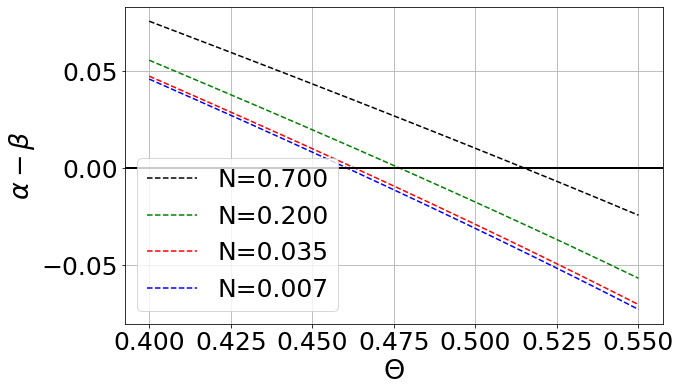
\includegraphics[scale=0.5]{alpha_minus_beta}
    \caption{Evolution of the difference between $\alpha$ and $\beta$ as a
    function of the cut value for different of feed assays, 0.007 (black),
    0.035 (red), 0.2 (green), 0.7 (black). }
    \label{fig_a_m_b}
\end{figure}

The number of machines required to construct a stage can then be computed using
equation \eqref{eq_alpha_principle} to solve for the centrifuge feed flow:

\begin{equation}\label{eq_cent_feed}
    F_c = \frac{2 \delta U}{(\alpha - 1)^2} \frac{M}{M_{238}} \frac{1-\theta}{\theta}
\end{equation}

Where the molar mass ratio $\frac{M}{M_{238}}$ accounts for the molar mass
differences between the feed gas, $UF_6$, and the individual uranium isotopes
being separated. The stage feed flow can then be divided by the individual
centrifuge feed flow, equation \eqref{eq_cent_feed}, to find the exact number of
machines needed for the ideal stage. In practice, this number is rounded up to
account for fractional machines required.


In a cascade, as the stage feed-to-product enrichment factor $\alpha_{i}$ and stage feed-to-tail enrichment factor $\beta_{i}$ remain constant, only the value of
the cut, $\theta_{i}$, changes across the different stages of a cascade.  This
algorithm assumes that the corresponding separative power $\delta U$ (not
re-computed) can be achieved with the chosen centrifuge design by tuning other
operational parameters such as the rotation speed, counter-current flow
ratio, etc.  Once $\theta_{i}$ is determined, it is possible to compute the
product and the tail assays.


The design of the ideal symmetric cascade is performed through 2 steps. First,
the configuration and number of stages is determined, adding stages with product assay $N'_i$ calculated using equation \ref{eq_product_assay}, until the
product assay of the final stage is greater than or equal to the product targeted assay. The stage tails assay $N''_i$ is calculated similarly, until it is less than or equal to the tails desired assay.  This determines the number of enriching and stripping stages as well as their enrichment properties ($N_{i}$, $N'_{i}$, $N''_{i}$,$\theta_{i}$).


The second step determines the relative flows at each stage, solving the linear
flow equation, \eqref{eq_flow}.
The cascade can then be populated with actual machines until the maximum number
of available machines is reached.

\begin{equation}
\resizebox{\linewidth}{!}{%
$\displaystyle
\setcounter{MaxMatrixCols}{20}
\begin{bmatrix}
     -1      & 1-\theta_{_{S+1}} & 0                 & ...  & 0            & 0            & 0             & 0             & 0             & ... & 0               & 0  & 0 \\
\theta_{_S}  & -1                & 1-\theta_{_{S+2}} & ...  & 0            & 0            & 0             & 0             & 0             & ... & 0               & 0  & 0 \\
             &                   &                   &      &              &              & ...           &               &               &     &                 &    &   \\
 0           & 0                 & 0                 & ...  & \theta_{_-2} & -1           & 1-\theta_{_0} & 0             & 0             & ... & 0               & 0  & 0 \\
 0           & 0                 & 0                 & ...  & 0            & \theta_{_-1} & -1            & 1-\theta_{_1} & 0             & ... & 0               & 0  & 0 \\
 0           & 0                 & 0                 & ...  & 0            & 0            & \theta_{_0}   & -1            & 1-\theta_{_2} & ... & 0               & 0  & 0 \\
             &                   &                   &      &              &              & ...           &               &               &     &                 &    &   \\
 0           & 0                 & 0                 & ...  & 0            & 0            & 0             & 0             & 0             & ... & \theta_{_{E-2}} & -1 & 1-\theta_{_E} \\
 0           & 0                 & 0                 & ...  & 0            & 0            & 0             & 0             & 0             & ... & 0               & \theta_{_{E-1}} & -1
 \end{bmatrix}
 \times
 \begin{bmatrix}
     F_{_{S}}   \\
     F_{_{S+1}} \\
     \cdots     \\
     F_{_{-1}}  \\
     F_{_{0} }  \\
     F_{_{1} }  \\
     \cdots     \\
     F_{_{E-1}} \\
     F_{_{E}}
 \end{bmatrix}
 =
 \begin{bmatrix}
     0      \\
     0      \\
     \cdots \\
     0      \\
     F      \\
     0      \\
     \cdots \\
     0      \\
     0
\end{bmatrix}
$}
%\caption{caption needed!}
\label{eq_flow}
\end{equation}



\subsection{Misuse models}

Little information is available about optimising an existing enrichment cascade
that is being fed with a feed enrichment that does not match the design
enrichment. Here, 3 different methods will be investigated.

The first method, A, assumes that no changes are being made to the cascade, i.e $\delta U$, $F$ and $\theta$ are fixed across all stages. The second method, B, assumes the cut value $\theta$ is re-tuned at each stage to maintain the ideal state of the cascade, while $\alpha$ and $\beta$ remain fixed. The last method, C, described in \cite{walker.2017} assumes the tails-to-product enrichment factor $\gamma$ and the cut $\theta$ remain constants
(eq. \eqref{eq_gamma-def}: $\gamma = \alpha\beta$). Model behaviors and
assumptions are summarized in Tab. \ref{tab:models}.

\begin{table}[htb]
\centering
  \caption{Summary of misuse model properties.}
\begin{tabular}{l|ccc}
\toprule

Model                &    A                 & B                  & C  \\
\midrule
Constant parameters  & $\alpha_i, \theta_i$ & $\alpha_i=\beta_i$ & $\gamma_i=\alpha_i\beta_i, \theta_i$       \\
Varying parameters   & $\beta_i$            & $\theta_i$         & $\alpha_i, \beta_i$                     \\
Assays determination & blended              & ideal              & blended                  \\
Flow                 & unchanged            & reduced            & unchanged       \\

\bottomrule
\end{tabular}
  \label{tab:models}
\end{table}

\subsubsection{Model A}

The tuning method A does not re-optimize $\theta_i$, keeping the same flow as the
ideal configuration. From equation \eqref{eq_alpha}, maintaining $\delta U$ and
$F$ while $\theta$ is unchanged implies $\alpha$ remains unchanged as well.
According to equation \eqref{eq_beta}, when $\alpha$ and $\theta$ are fixed, if
the feed assay ($N$) changes, $\beta$ will change accordingly.  This breaks the
ideal status of the cascade, i.e. $N_{i} \neq N'_{i-1} \neq N''_{i+1}$.


In order to compute the proper product and tails assay at each stage, the tail
and the product from the next and the previous stage respectively must be
blended in order to determine the correct stage feed assay. All feed assays are
iteratively updated, blending the proper product and tails, then using the
updated feed assay, the new product and tails assays are recomputed. This
process is repeated until the sum of the square difference in assays is smaller
than $10^{-8}$.  As the cut remains fixed at each stage, the flows do not need
to be recomputed.

This model assumes that it is possible to maintain the separative power of a
centrifuges, $\delta U$, for any feed assays $N$ while maintaining its cut
$\theta$ and feed flow $F$.

\subsubsection{Model B}

Using the second method, the cut value at each stage, $\theta_i$, is retuned in
order to maintain the $\alpha_i$ and $\beta_i$ at their original values
(equation \eqref{eq_theta}). Since the cascade remains ideal, the product and
tails assay at each stage can easily be determined using equations
\eqref{eq_alphabeta}.

As the cut values change, the relative flow rates between the different stages
are recomputed using equation \eqref{eq_flow}.  Under this model, the flow at
each stage of the original ideal cascade is assumed to be the maximum flow
allowed at that stage.  Therefore, all of the recomputed flow rates are scaled
together to ensure that no stage experiences a flow rate larger than that of
the original cascade.  Some stages may now experience flow rates much lower
than the original cascade.

%% The flow rates are determinted as
%% the largest flow rates allowed by the cascade design, number of centrifuges
%% limiting the flow at each stage.

This model assumes that it is possible to tune a centrifuge separative power
$\delta U$, for any feed assay $N$, cut $\theta$ and feed flow $F$, in order to
maintain its constant feed to product enrichment factor $\alpha$.




\subsubsection{Model C}
The last model assumes that the tails to product enrichment factor remains
constant regardless to the feed assays. To compute the response of the cascade
one need to determine $\alpha$ and $\beta$ such that their product and
$\theta$ remain fixed.
From equations \eqref{eq_alphabeta} and the assay conservation equation $N =
\theta N' + (1-\theta)N''$ it is possible to express the product, $N'$,
dependent on the feed assay $N$, $\gamma$, and the cut, $\theta$, as one
solution of the second order equation \eqref{eq_gamma_p}:

\begin{equation}\label{eq_gamma_p}
    \theta(\gamma-1)N'^2+((N+\theta)(\gamma-1)+1)N'-N\gamma = 0
\end{equation}


The only solution allowing product assay to range between 0 and 1 is the
following :

\begin{equation}\label{eq_model_b_sol}
    N' = \frac{N+\theta}{2\theta} +
         \frac{1 - \sqrt{\gamma^{2}(N-\theta)^{2}
                         + 2\gamma( N^{2} + N - \theta^{2} + \theta)
                         + (N + \theta + 1)^{2}}}
              {2\theta(\gamma - 1)}
\end{equation}

Once the product assay is known, one can trivially determine the tails assay,
$\alpha$ and $\beta$, using equations \eqref{eq_alphabeta} and mass
conservation.

Similar to model A, because the cut values remain constant, the flows do not
need to be recomputed and the correct assays, $\alpha$ and $\beta$, are
determined through iterative blending of the product assays of the previous
stage and the tails assay of the next stage using equation
\eqref{eq_model_b_sol}.

This model assumes that it is possible to tune the centrifuge separative power
$\delta U$ in order to maintain for any feed assay $N$ and its tails to product
enrichment factor $\gamma$ while maintaining its cut $\theta$ and feed flow $F$.

%The speed at which each models reach a threshold of $90\%$ enrichment is
%illustrated in Figure \ref{fig:model_comparison}. The production curve of
%enrichment for each model is shown. The step functions for each model represent
%the cascade configuration. Each step is one cascade in a chain of cascades and
%the shape of the curve for each model gives an indication of how quickly the model
%can reach the enrichment threshold. The main difference is that Model B reaches
%the threshold faster, whereas Models A and C reach a higher enrichment value.
%This highlights some of the immediate differences that would influence the choice
%of using each model in a breakout scenario.

%\begin{figure}[ht]
%    \centering
%    \includegraphics[scale=0.4]{ModelComparison}
%    \caption{The curve of resulting product assays for each model is plotted.
%    Since the feed assay of each cascade is fed into the next cascade in the
%    chain, a linear relationship between the product and feed assays is plotted
%    in black. The step function for each model represents the output of the
%    cascade chain (each step is a cascade). While there are four steps for each
%    model, Model B (green) reached the $90\%$ enrichment threshold before
%    Model A (red) or Model C (blue). However, in the same amount of steps, Models
%    A and C are able to achieve a higher enrichment percent than Model B.}
%    \label{fig:model_comparison}
%\end{figure}


% III. Experiement
%   a.  cycle 
%   b.  cascade per level optimisation
\section{The experiment}
This work focuses on comparing the different misuse models to a reference
calculation in which a single large cascade is designed and built to directly
produce \gls{HEU} from natural uranium.
This works uses the Cyclus fuel cycle simulator to allow material exchange
between facilities. The enrichment cascade algorithm has been implemented in
the $mbmore$ package \cite{mbmore.2018}.
In each cases, 5060 centrifuges have been used and spread across up to 30
different gas centrifuge enrichment cascades. This is inspired by limitations
placed on the Iranian uranium enrichment program via the Joint Comprehensive
Plan of Action (JCPoA) \cite{jcpoa}.


\subsection{The cascade configuration}

\subsubsection{Reference}

As mentioned, all the further calculations will be compared to the most
favorable configuration to produce \gls{HEU}, where all the available
centrifuges are used in a single large ideal symmetric cascade designed to
directly produce \gls{HEU} from natural uranium, with a tails assay close to
$0.3w\%$. The design characteristic of the reference cascade are summarized in
Table \ref{tab:cascade_config}.

\subsubsection{Default cascade}

The default cascade is the ideal symmetric cascade designed for normal civilian
enrichment operation, enriching natural uranium to about $3.5w\%$, with a tails
assay close to $0.3w\%$. This cascade will be layered and fed with uranium at
higher enrichment to evaluate the possibility to use them, with little or no
tuning, to produce \gls{HEU}. The characteristics of the default cascade are
summarized in Table \ref{tab:cascade_config}.

\begin{table}[htb]
\centering
  \caption{Summary of cascade design.}
\begin{tabular}{cccc}
\toprule

Cascade Design &       & Reference   & Default    \\
\midrule
Targeted  & Feed       & $0.71w\%$   & $0.71w\%$  \\
Assays    & Product    & $90w\%$     & $3.5w\%$   \\
          & Tails      & $0.3w\%$   & $0.3w\%$   \\
\midrule
Effective & Product    & $90.35w\%$  & $4.13w\%$  \\
Assays    & Tails      & $0.29w\%$   & $0.29w\%$  \\ 
\midrule
Stages    & Stripping  & 4          & 4          \\
Number    & Enriching  & 39         & 10         \\
\bottomrule
\end{tabular}
  \label{tab:cascade_config}
\end{table}


\subsection{Scenarios}
In the following, cascades can be connected in tandem, where each set of cascade
in parallel is called a ``level``, as illustrated in Figure
\ref{fig:cascade_level}.
The reseults from seven different simulations have been compared, to evaluate the effectiveness
of an enrichment cascade when used outside of its designed scope :
\begin{itemize}
\item one as the reference calculation, with a single cascade designed to
    directly produce \gls{HEU} from natural uranium,
\item three calculations (one per misuse model) where default cascade are
    chained to produce \gls{HEU}, without recycling the tails of each cascade
    sending their tails to the waste,
\item three calculations (one per misuse model) where default cascade are
    chained to produce \gls{HEU}, and the tails of each cascade are recycled, blending
    the tails of one level in the feed of the previous level of
    cascades (see Figure \ref{fig:cascade_level}).
\end{itemize}

\begin{figure}[ht] % replace 't' with 'b' to force it to be on the bottom
    \centering
    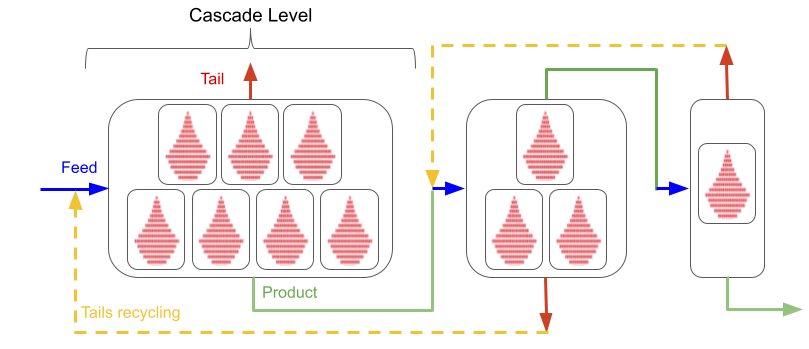
\includegraphics[width=\linewidth]{flow}
    \caption{Schematic representation of the chained cascades with three levels,
    with the feed, product and the tails flows, in blue, green and red,
    respectively. The dashed orange line represent the alternative tails flow when
    tails recycling is considered.}
    \label{fig:cascade_level}
\end{figure}


\subsection{Level population}
In order to assign the optimum number of cascades to each level, a ``level cut'' as
been computed as:
\begin{equation}
    \Omega_{j} = \frac{N_{j}-N''_{j}}{N'_{j}-N''_{j}},
\end{equation}
where, $j$ represents a level of cascade and $N_{j}$, $N'_{j}$ and $N''_{j}$
the feed, product and tails assay, respectively, of the cascades at this level.

A flow equation similar to \eqref{eq_flow} is then solved to obtain the optimum
number of cascade per level. When the tails are not recycled, the $(1-\theta)$
terms are removed from the flow equation.  The results of the level population
are summarized in Table \ref{tab:level}.

As it is not possible to assign a fraction of an enrichment cascade, cascade per
level must be rounded and assigned for each level. Again, per the JCPoA, 30
cascades are distributed to the appropriate number of levels to achieve an
HEU threshold with the least amount of levels. This optimal assignment is
manually tested by running many different configurations. In generally, each
level besides the first is rounded up from its optimal fractional value, with
the remaining cascades being assigned to the first level.


%% \subsection{Timestep effect}
%% 
%% The different cascade levels required up to $2n+1$ timesteps
%% before it starts to enrich uranium, where $n$ corresponds to the level number.
%% This corresponds to the number of timesteps required for the material to
%% propagate from the natural uranium source to the $n$-th level, regardless of the
%% duration of the timestep (hour, day, month, etc.). This is also true for the
%% number of timesteps required to reach the equilibrium assays value in the tails
%% reprocessing cases.  As timestep can be artificially small or large, one will
%% only be considering equilibrium values of flow rates and assays in the following
%% analysis.


% IV.  results
%   a. time step effects
%   b. no tails recycling
%   c. tails recycling
\section{Results}

\subsection{Miss-use modeling}

\begin{table}[h!]
\footnotesize
\centering
  \caption{Summary of cascades level population.}
\resizebox{\columnwidth}{!}{%
\begin{tabular*}{\linewidth}{c @{\extracolsep{\fill}} cccccccc}
\toprule

Model       &        &                & A/NR     & A/R      & B/NR     & B/R      & C/NR     & C/R       \\
%Recycling   &       &                & No       & Yes      & No       & Yes      & No       & Yes        \\
\midrule                                                                                                 
        &            & Feed $w\%$     & $0.71$   & $1.31$   & $0.71$   & $0.92$   & $0.71$   & $1.30$ \\
Level 0 & Assay      & Product $w\%$  & $3.97$   & $7.27$   & $3.97$   & $5.10$   & $3.97$   & $7.24$ \\
        &            & Tails $w\%$    & $0.28$   & $0.52$   & $0.28$   & $0.36$   & $0.28$   & $0.51$ \\
        & Cascades   & Impl. (Ideal)  & 25(26.5) & 25(26.5) & 24(26.4) & 25(26.3) & 25(26.5) & 25(26.2)  \\
\midrule                                                                                                 
        &            & Feed $w\%$     & $3.97$   & $11.48$  & $3.97$   & $6.29$   & $3.97$   & $11.64$ \\
Level 1 & Assay      & Product $w\%$  & $21.29$  & $53.30$  & $19.33$  & $27.98$  & $21.41$  & $55.12$ \\
        &            & Tails $w\%$    & $1.68$   & $5.93$   & $1.58$   & $2.54$   & $1.66$   & $5.88$ \\
        & Cascades   & Impl. (Ideal)  & 3(3.1)   & 4(3.1)   & 3(3.1)   & 3(3.1)   & 3(3.1)   & 4(3.4)    \\
\midrule                                                                                                 
        &            & Feed $w\%$     & $21.29$  & $53.3$   & $19.33$  & $31.09$  & $21.41$  & $55.12$ \\
Level 2 & Assay      & Product $w\%$  & $76.39$  & $94.70$  & $58.10$  & $72.31$  & $79.21$  & $96.37$ \\
        &            & Tails $w\%$    & $13.98$  & $47.81$  & $8.51$   & $14.91$  & $13.75$  & $49.65$ \\
        & Cascades   & Impl. (Ideal)  & 1(0.4)   & 1(0.4)   & 1(0.4)   & 1(0.5)   & 1(0.4)   & 1(0.4)   \\
\midrule                                                                                                 
        &            & Feed $w\%$     & $76.39$  & N.A.     & $58.10$  & $72.31$  & $79.21$  & N.A.      \\
Level 3 & Assay      & Product $w\%$  & $98.09$  & N.A.     & $88.92$  & $93.79$  & $98.86$  & N.A.      \\
        &            & Tails $w\%$    & $73.51$  & N.A.     & $35.01$  & $50.36$  & $76.60$  & N.A.      \\
        & Cascades   & Impl. (Ideal)  & 1(0.04)  & N.A.     & 1(0.09)  & 1(0.1)   & 1(0.04)  & N.A.      \\
\midrule                                                                                                 
        &            & Feed $w\%$     & N.A.     & N.A.     & $88.92$  & N.A.     & N.A.     & N.A.      \\
Level 4 & Assay      & Product $w\%$  & N.A.     & N.A.     & $97.89$  & N.A.     & N.A.     & N.A.      \\
        &            & Tails $w\%$    & N.A.     & N.A.     & $75.71$  & N.A.     & N.A.     & N.A.      \\
        & Cascades   & Impl. (Ideal)  & N.A.     & N.A.     & 1(0.04)  & N.A.     & N.A.     & N.A.      \\
\bottomrule
\end{tabular*}
}
\label{tab:level}
\end{table}

As illustrated in Figures \ref{fig:assays} and summarized on Table
\ref{tab:level}, the different models don't have the same effect on the
cascade behavior. While models A and C achieve a quick enrichment gain with
the cascades chaining, 4/21/76/98 and 4/21/79/99, respectively, model B only
achieves an enrichment gain of 4/19/58/89/98, requiring more levels to even
achieve HEU enrichment. This table also shows the integer
number of cascades implemented (Impl.) at each level in the simulation, compared
to the non-integer number of cascades that would achieve an ideal configuration (Ideal).


\begin{figure}[h!]
    \centering
    \begin{subfigure}[t]{0.45\textwidth}
        \centering
        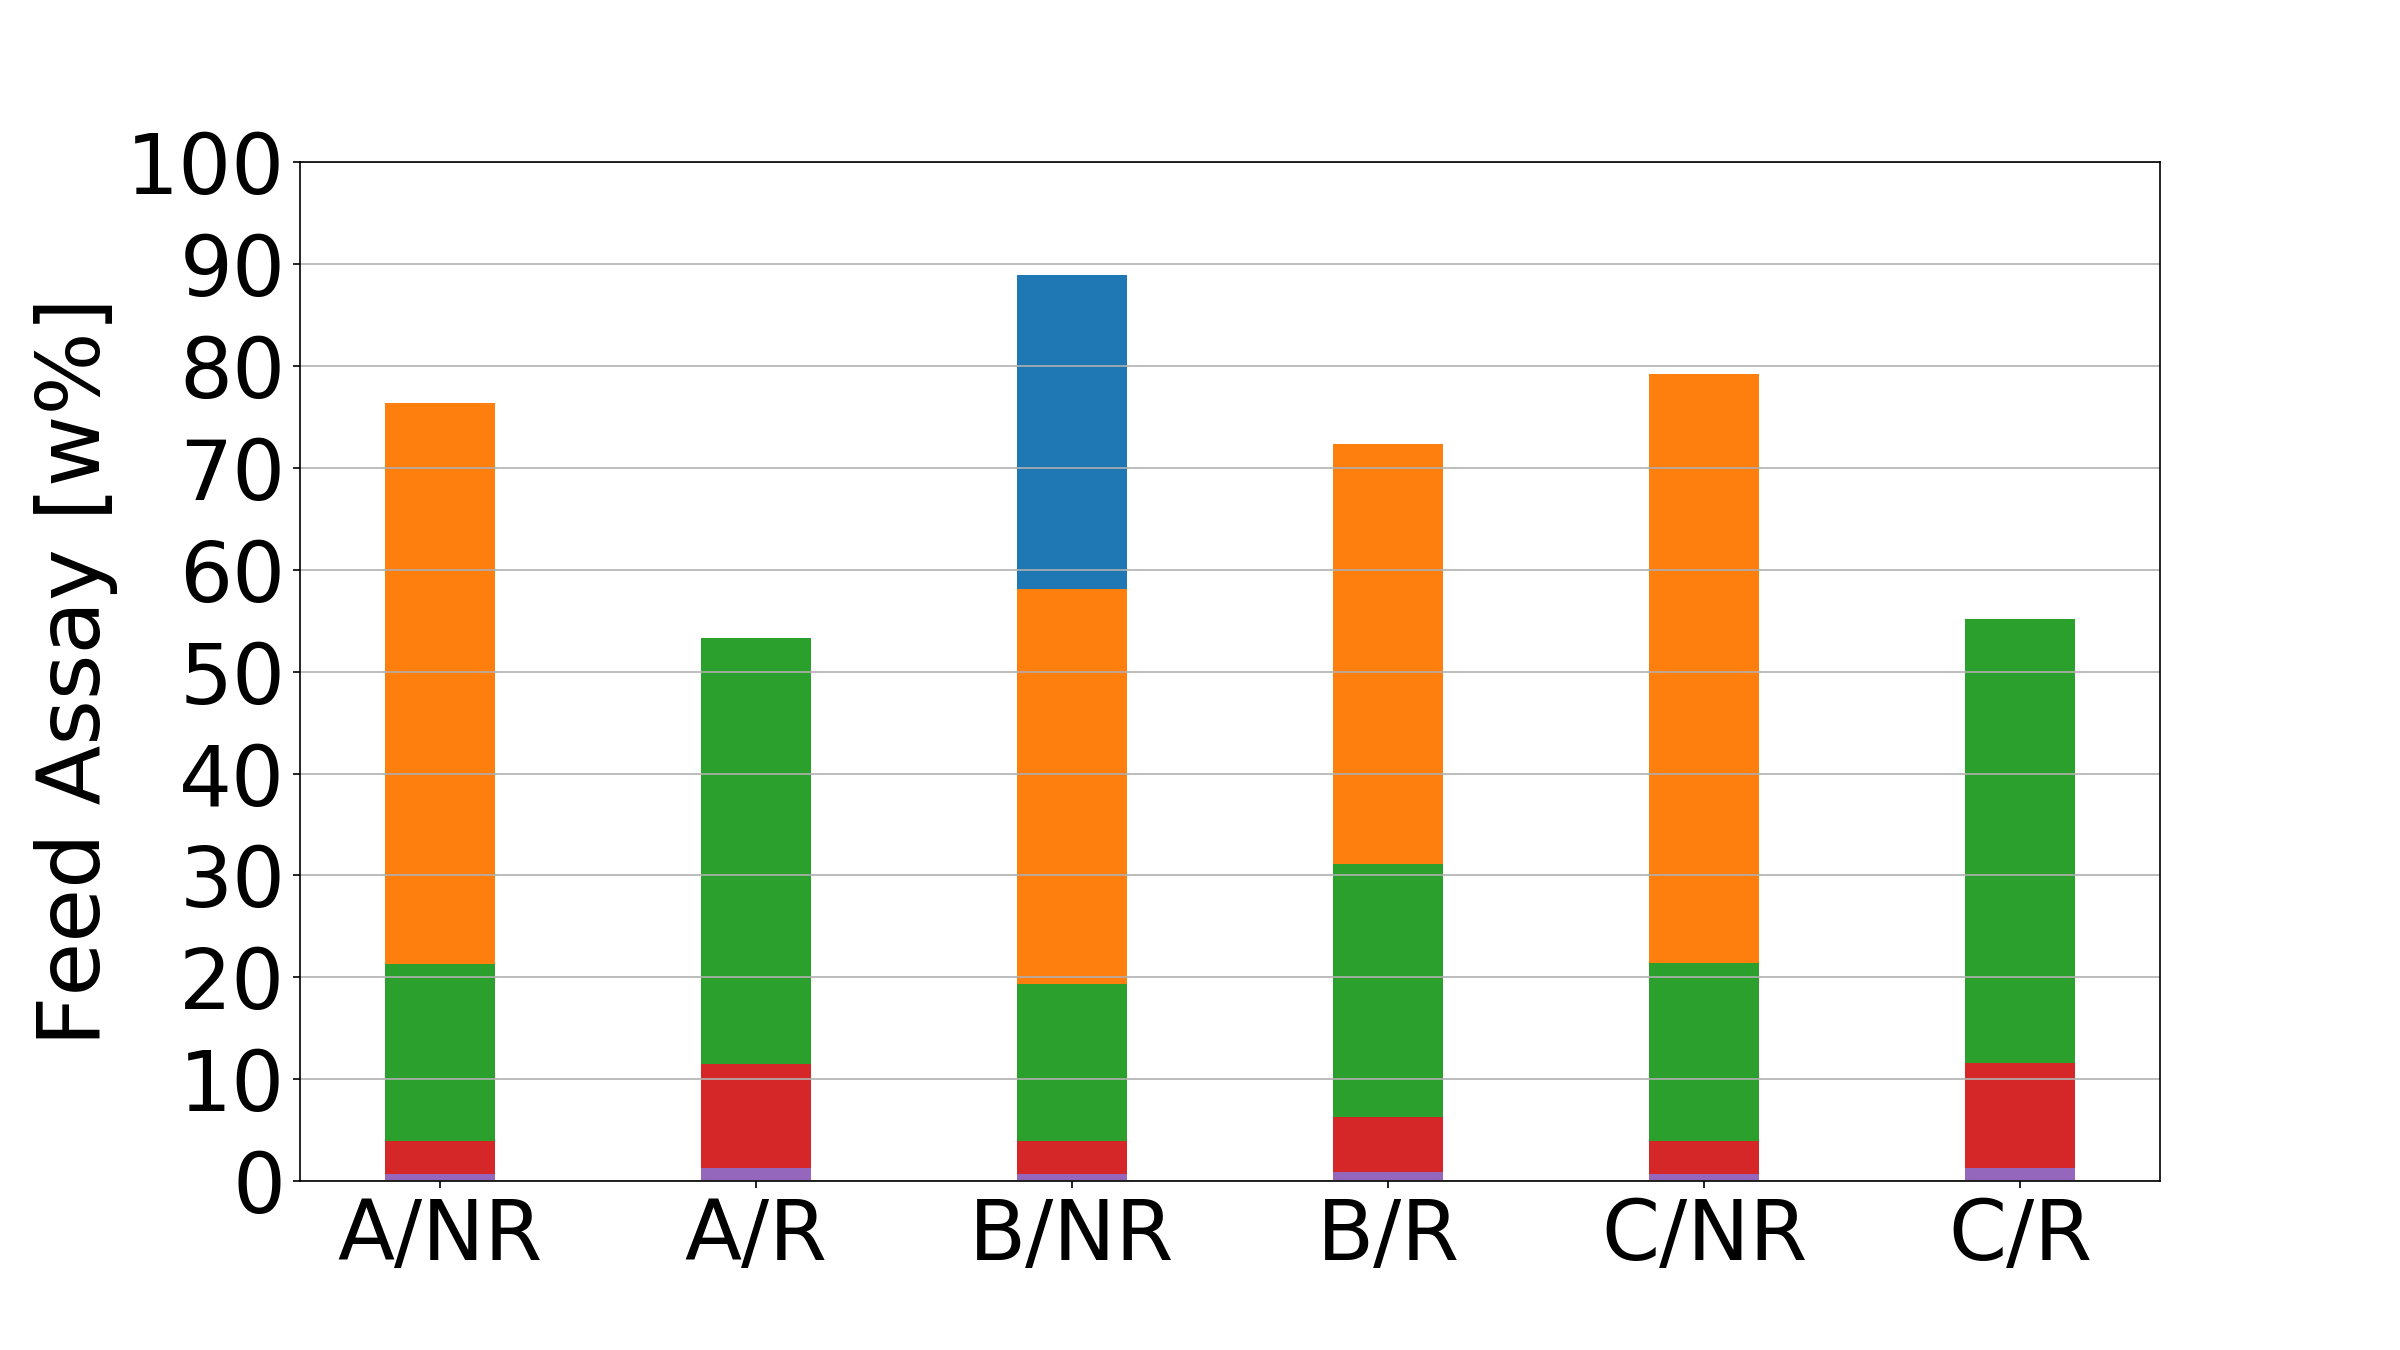
\includegraphics[width=\linewidth]{feed_assays}
        \caption{Feed Assays}
        \label{sfig:feed_assay}
    \end{subfigure}%
    \begin{subfigure}[t]{0.45\textwidth}
        \centering
        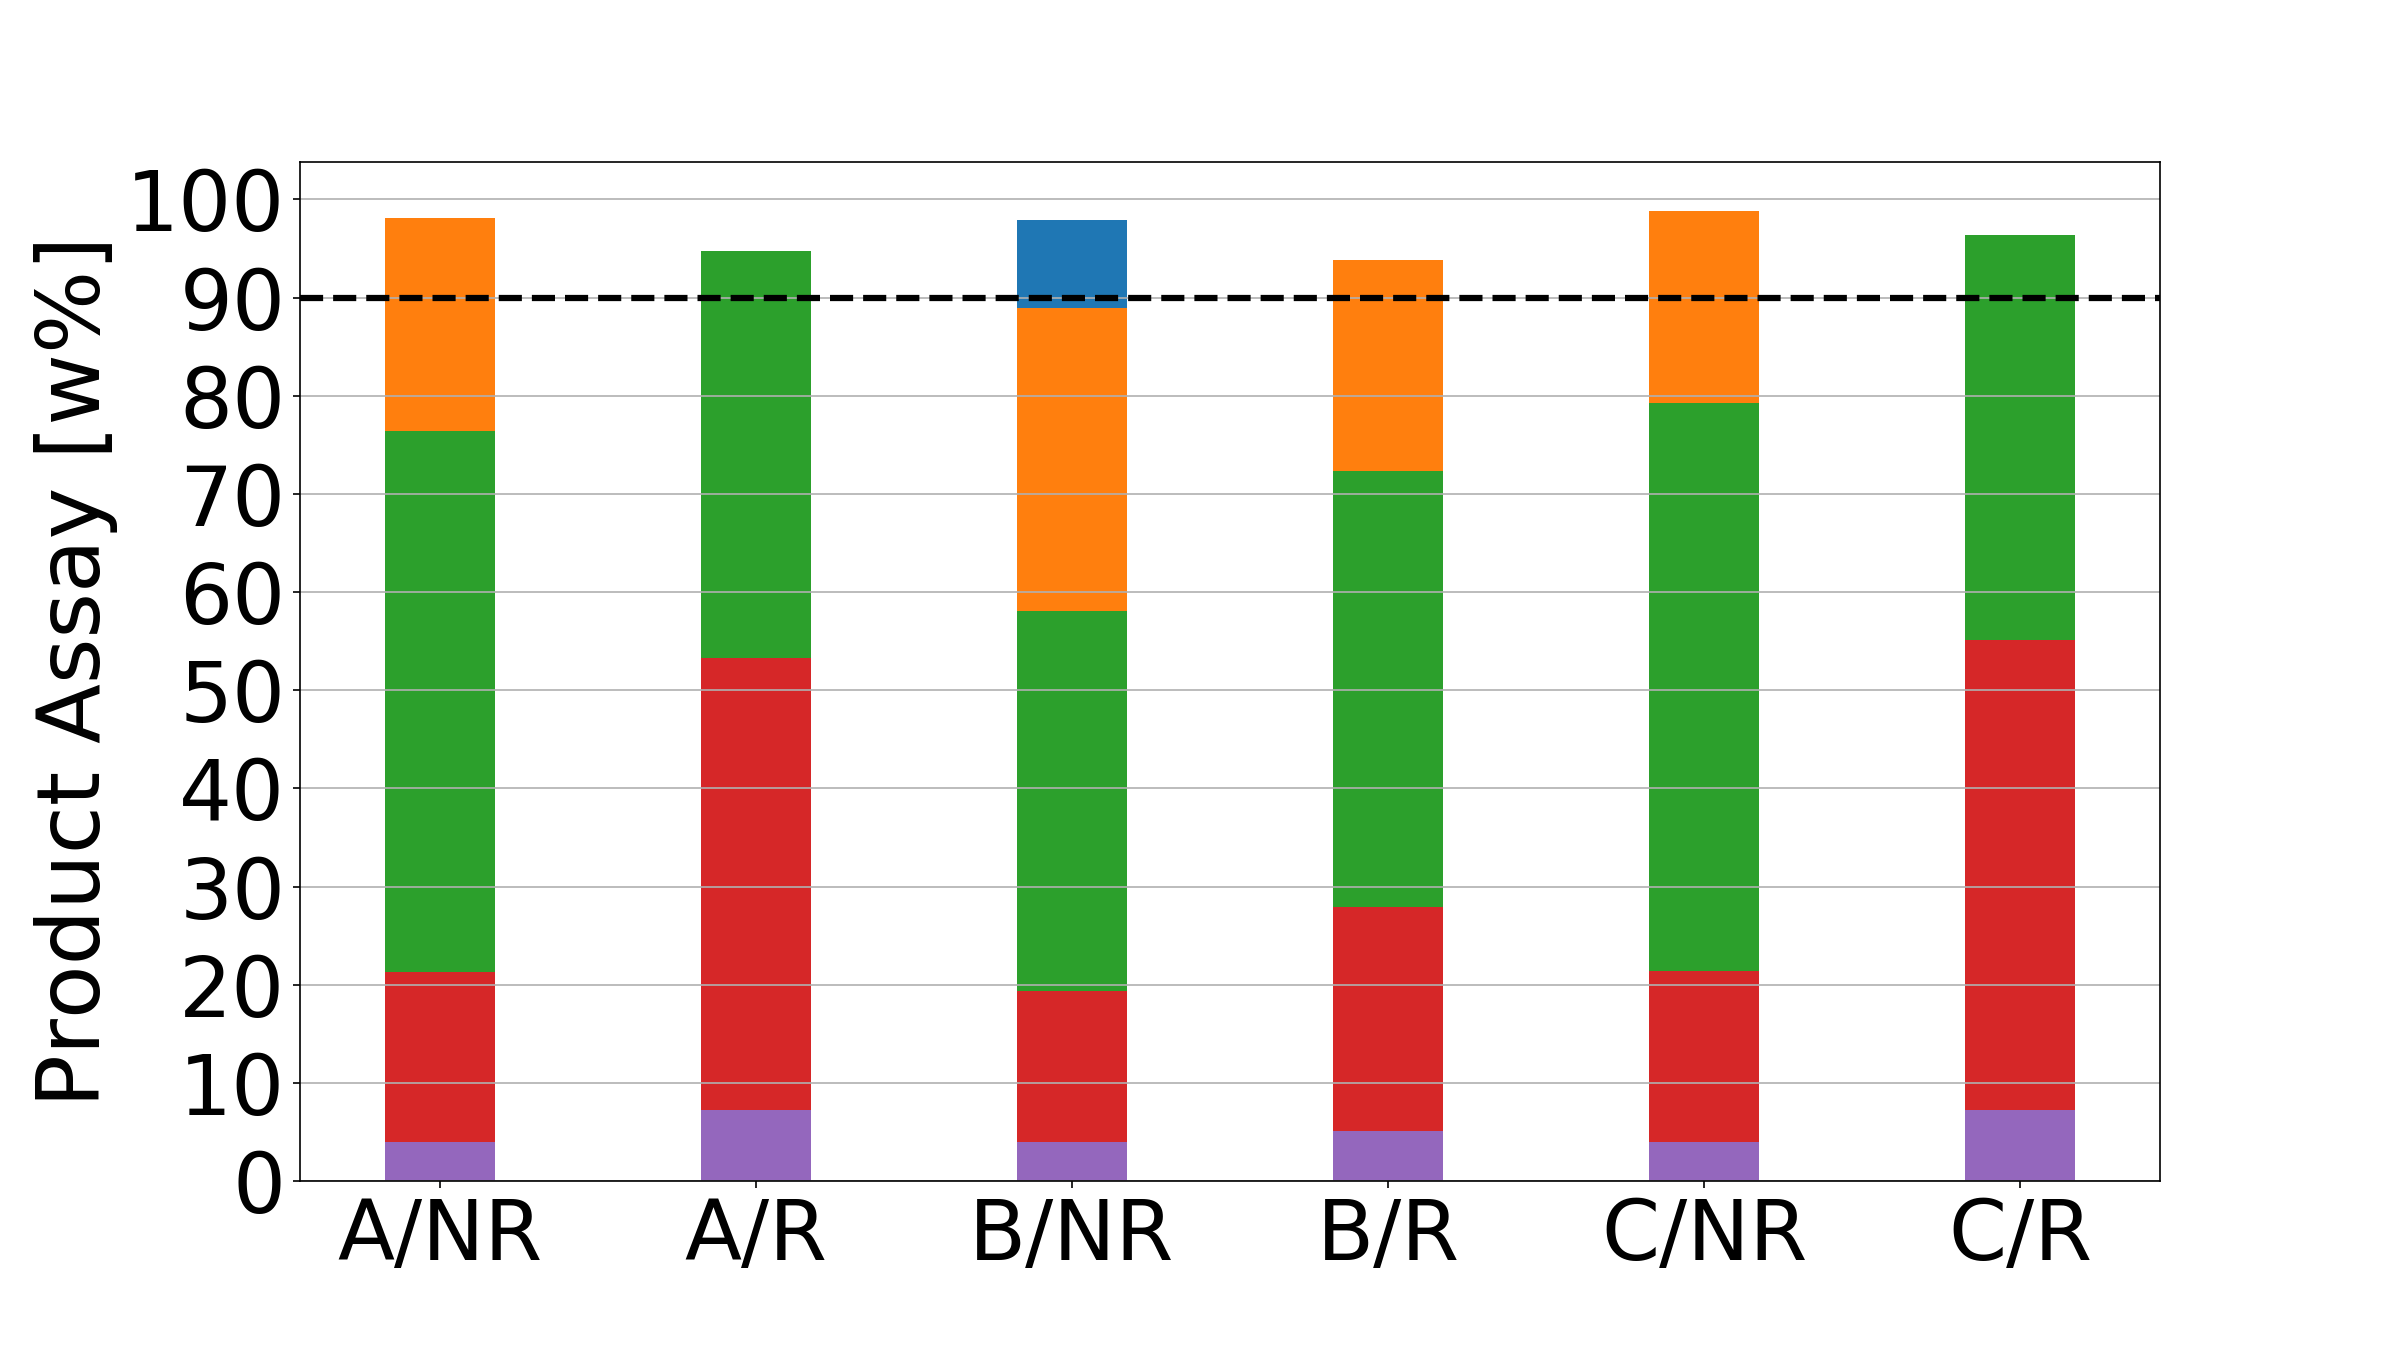
\includegraphics[width=\linewidth]{product_assays}
        \caption{Product Assays}
        \label{sfig:product_assay}
    \end{subfigure}
    \begin{subfigure}[t]{0.45\textwidth}
        \centering
        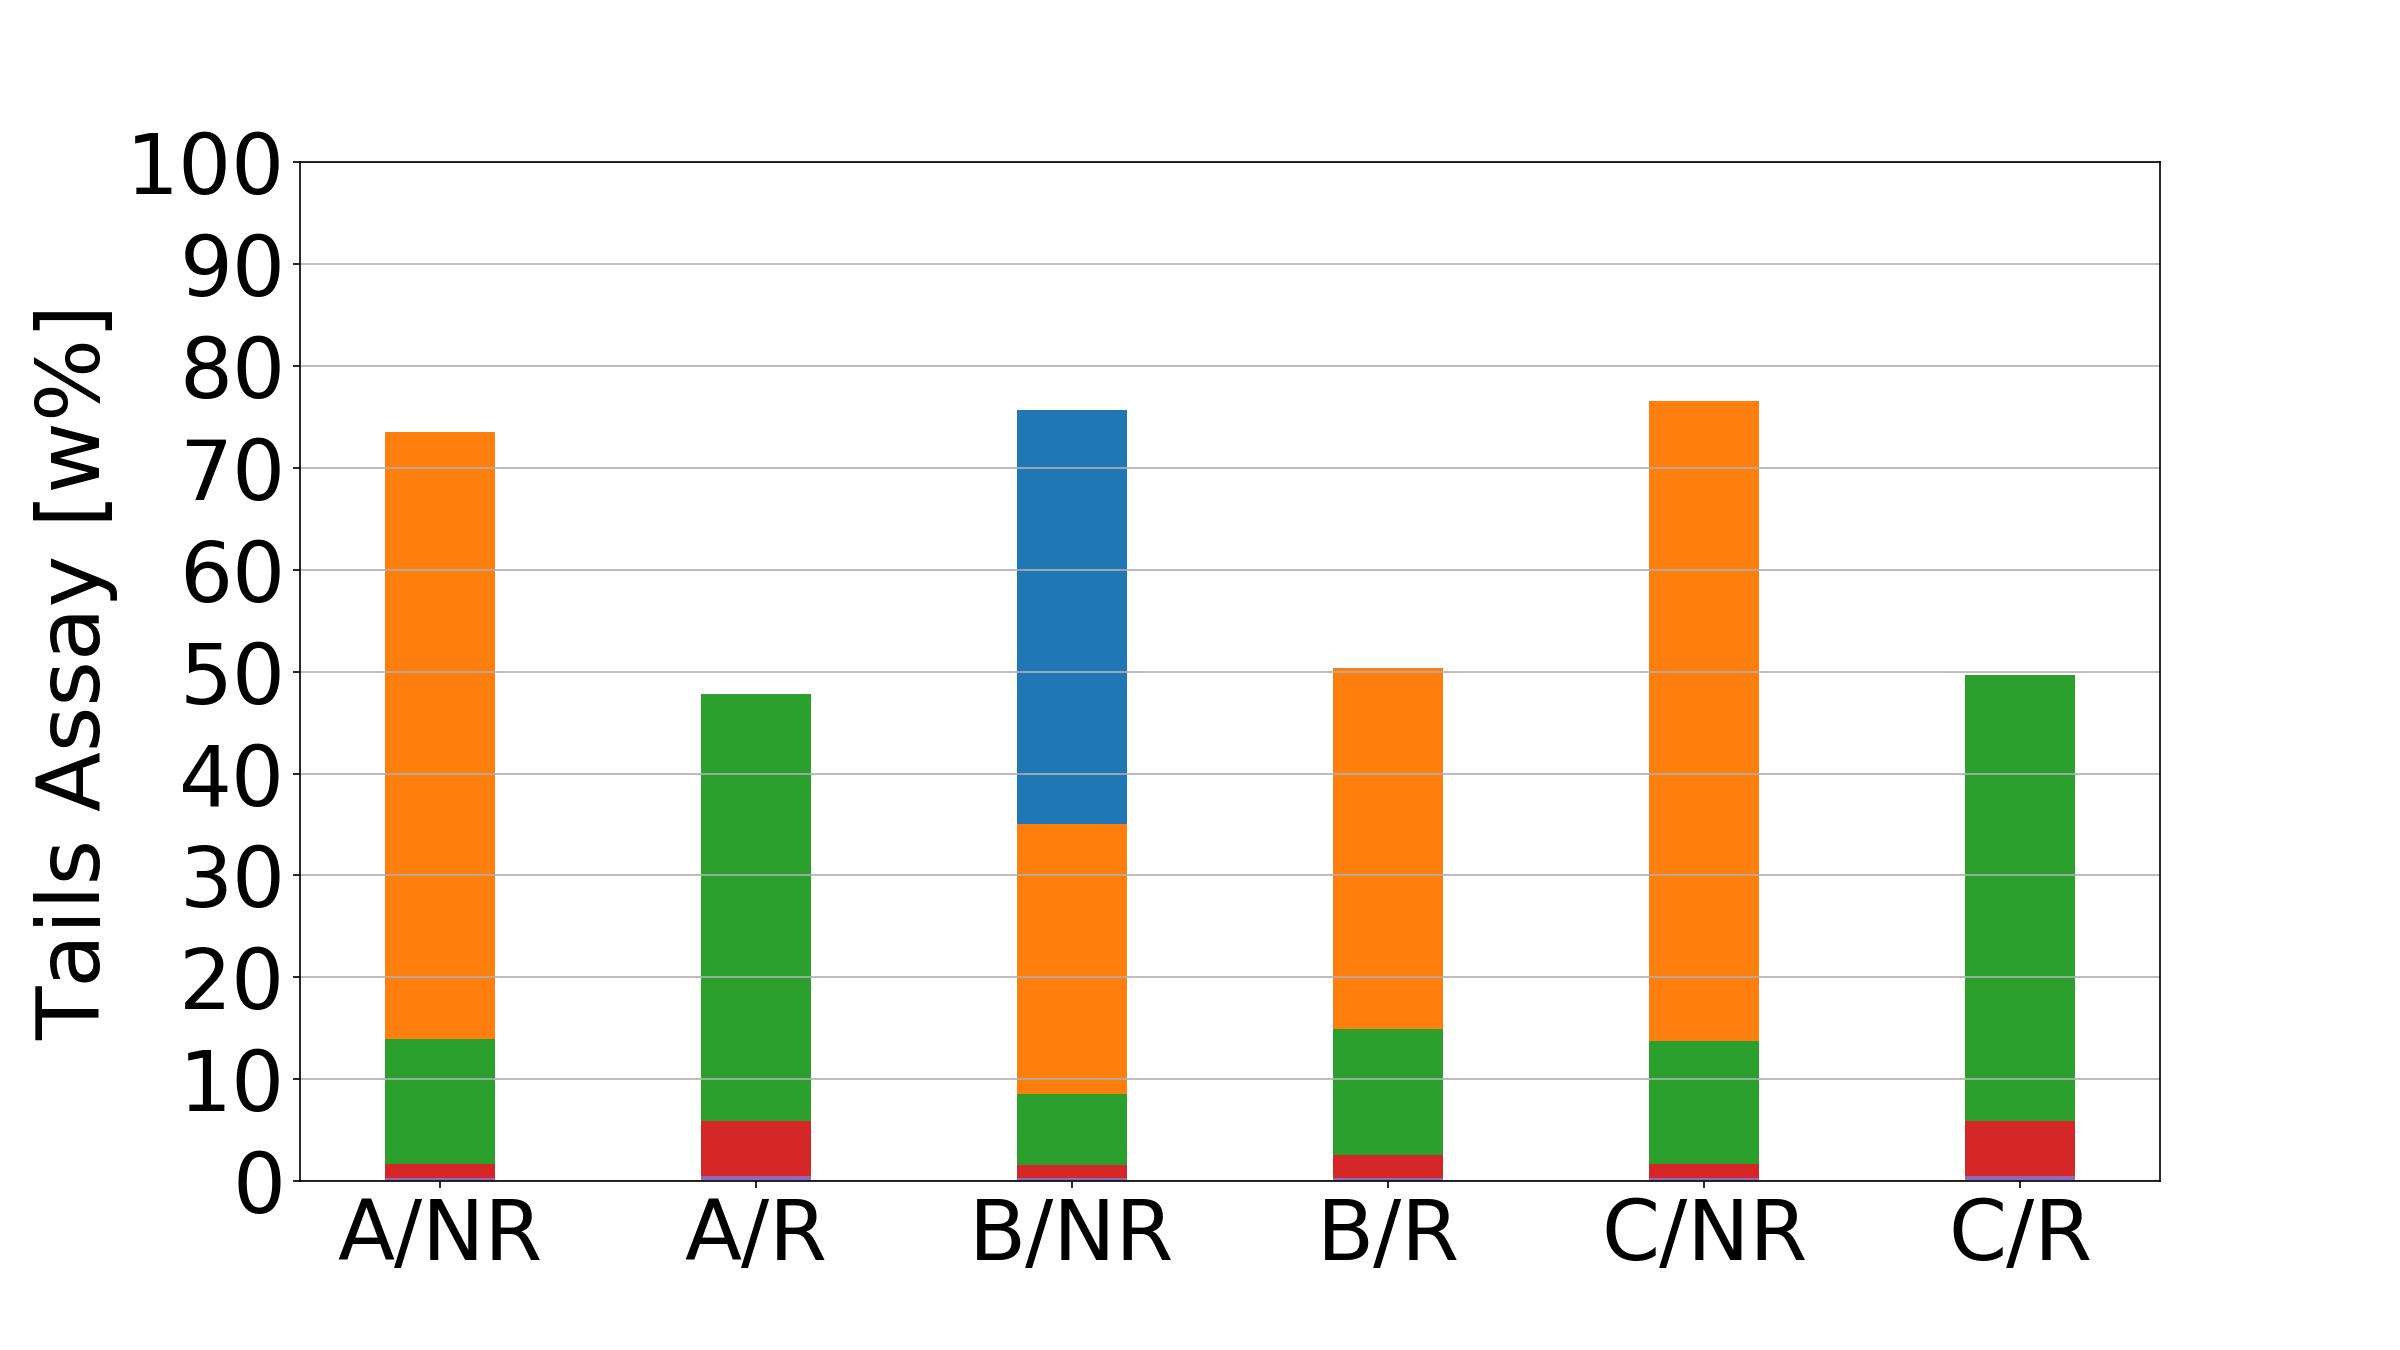
\includegraphics[width=\linewidth]{tails_assays}
        \caption{Tails Assays}
        \label{sfig:tails_assay}
    \end{subfigure}
    \caption{Feed (\subref{sfig:feed_assay}), product
        (\subref{sfig:product_assay}) and tails assays (\subref{sfig:tails_assay})
        in $w\%$ of $^{235}$U, per cascade level from 0 to 4 (purple, red, green,
        orange, blue), per model (A/B/C) and without/with tails recycling (NR/R).
        The black dashed line represents the $90 w\%$ enrichment threshold.}
    \label{fig:assays}
\end{figure}



\subsection{Tails recycling}

As shown in Figures \ref{fig:assays}, recycling the tails increases the overall product assay at
all the different levels, requiring less levels in the configuration to achieve
the desired enrichment. As the tails assay of a level $n+1$ is always higher than
the product assay of the level $n-1$, recycling the tails of level $n+1$ will
consequently increase the feed assay of level $n$ (see Table \ref{tab:level}).
Moreover, with an increased feed assay, tails and product assays increase as
well, increasing de facto the feed assays of respective cascade levels $n-1$
and $n+1$, etc.  This effect reduces the number of cascade levels required to reach
\gls{HEU} in all cases.



\subsection{\gls{HEU} Production Rate}

As shown in Figure \ref{fig:HEU_rate}, recycling increases the final \gls{HEU}
production rate, from $5$ to almost $45$ kg/y when using models A and C, and from
$12$ to $45$ kg/y with the model B. For the reference calculation, where all the
available cascades are used within a single large cascade design for direct
\gls{HEU} production, the \gls{HEU} production rate is slightly over $60$ kg/y.


As models A and C rely on maintaining the cut values at each stage of the
cascade and share the same number of levels, they have the exact same cascade
repartition across the different levels and the same \gls{HEU} production rate.

\begin{figure}[h!] % replace 't' with 'b' to force it to be on the bottom
    \centering
    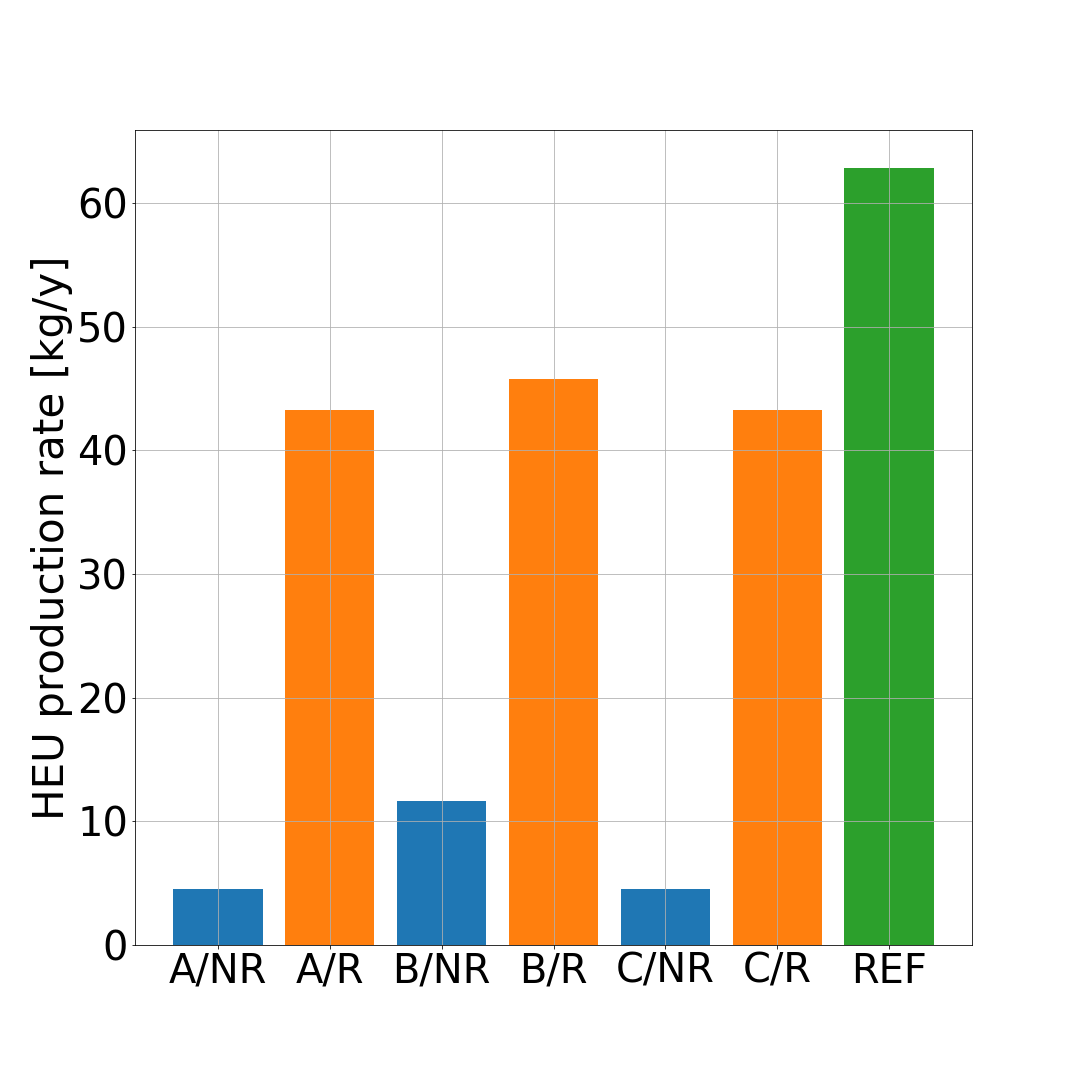
\includegraphics[scale=0.25]{HEU_prod_rate}
    \caption{Production rate at equilibrium for the different model
        configurations, the case without tails recycling (blue), with tails
        recycling (orange), and the reference one (green). A-B-C represent
        the model used, and NR-R the case without tails recycling and the case
        with tails recycling, respectively.}
    \label{fig:HEU_rate}
\end{figure}


% V.  Discussion
% VI. Conclusions and future plan
\section{Discussion}

We can observe that when the cascade is left completely untouched (Model A) or
when it is slightly retuned to maintain the tails to product enrichment factor
as well as the cut of each centrifuges (Model C), chaining the cascade can
achieve large increase of the enrichment at each level.  On the contrary, when
retuning the cut of each centrifuge to maintain the ideal state of the cascades
(Model B) while chaining them, the \gls{HEU} production rate is favored over the
enrichment gain.

The tails recycling allows each model to achieve a large gain in productivity.
Even if no cascade chaining options achieves the same production rate as direct
enrichment, all models with tail recycling reached close to $73\%$ of the optimum
production rate. Such a production rate would allow the accumulation of a
Significant Quantity of \gls{HEU} in less than 8 months\ldots


\section{Conclusion and future work}

This work has investigated the possibility to chain centrifuge enrichment
cascades that are designed to enrich uranium for commercial reactors in order to
produce \gls{HEU} instead. Three methods have been implemented to model
symmetric enrichment cascade behavior when fed with different uranium enrichment
than designed. 

%% This work has investigated and quantified the difference between potential
%% models for retuning of a centrifuge enrichment cascade in order to chain them to produce
%% \gls{HEU} initially tuned to produce uranium enrichment for commercial reactors.
Each method achieves up to $73\%$ of the production rate of a single
large enrichment cascade designed specifically for \gls{HEU} production using
the same number of centrifuges.

This work will be extended to the near future with additional misuse methods,
allowing for example, the reconfiguration of the centrifuges in the cascades.

For this study, the use of the Cyclus fuel cycle simulator was not required;
it only allows a quick determination of the blending equilibrium. Future
studies will make use of the full capability of Cyclus Dynamic Resource
Exchange in order to automatically assign the different cascades to the
different level as function of the resources availability, optimising the
productions rates in each cases.

While mathematically correct, the authors do not guaranty the feasibility of the
different misuse tuning methods implemented and are welcoming any insight on the
matter.





\section{Acknowledgments}
This work was funded by the Consortium for Verification Technology under
Department of Energy National Nuclear Security Administration award number
DE-NA0002534

%\end{frontmatter}


%\input{appendix}

%%%%%%%%%%%%%%%%%%%%%%%%%%%%%%%%%%%%%%%%%%%%%%%%%%%%%%%%%%%%%%%%%%%%%%%%%%%%%%%%
\begin{small}
\bibliography{refs}  % NO SPACES BETWEEN BIB FILENAMES!
\end{small}
\end{document}
